%%%%%%%%%%%%%%%%%%%%%%%%%%%%%%%%%%%%%%%%%
% Beamer Presentation
% LaTeX Template
% Version 1.0 (10/11/12)
%
% This template has been downloaded from:
% http://www.LaTeXTemplates.com
%
% License:
% CC BY-NC-SA 3.0 (http://creativecommons.org/licenses/by-nc-sa/3.0/)
%
%%%%%%%%%%%%%%%%%%%%%%%%%%%%%%%%%%%%%%%%%

%----------------------------------------------------------------------------------------
%	PACKAGES AND THEMES
%----------------------------------------------------------------------------------------

\documentclass[aspectratio=169]{beamer}

\mode<presentation> {

% The Beamer class comes with a number of default slide themes
% which change the colors and layouts of slides. Below this is a list
% of all the themes, uncomment each in turn to see what they look like.

%\usetheme{default}
%\usetheme{AnnArbor}
%\usetheme{Antibes}
%\usetheme{Bergen}
%\usetheme{Berkeley}
%\usetheme{Berlin}
%\usetheme{Boadilla}
%\usetheme{CambridgeUS}
%\usetheme{Copenhagen}
%\usetheme{Darmstadt}
%\usetheme{Dresden}
%\usetheme{Frankfurt}
%\usetheme{Goettingen}
%\usetheme{Hannover}
%\usetheme{Ilmenau}
%\usetheme{JuanLesPins}
%\usetheme{Luebeck}
\usetheme{Madrid}
%\usetheme{Malmoe}
%\usetheme{Marburg}
%\usetheme{Montpellier}
%\usetheme{PaloAlto}
%\usetheme{Pittsburgh}
%\usetheme{Rochester}
%\usetheme{Singapore}
%\usetheme{Szeged}
%\usetheme{Warsaw}

% As well as themes, the Beamer class has a number of color themes
% for any slide theme. Uncomment each of these in turn to see how it
% changes the colors of your current slide theme.

%\usecolortheme{albatross}
%\usecolortheme{beaver}
%\usecolortheme{beetle}
%\usecolortheme{crane}
%\usecolortheme{dolphin}
%\usecolortheme{dove}
%\usecolortheme{fly}
%\usecolortheme{lily}
%\usecolortheme{orchid}
%\usecolortheme{rose}
%\usecolortheme{seagull}
%\usecolortheme{seahorse}
%\usecolortheme{whale}
%\usecolortheme{wolverine}

%\setbeamertemplate{footline} % To remove the footer line in all slides uncomment this line
%% \setbeamertemplate{footline}[page number] % To replace the footer line in all slides with a simple slide count uncomment this line

\setbeamertemplate{navigation symbols}{} % To remove the navigation symbols from the bottom of all slides uncomment this line
}

\usepackage{graphicx} % Allows including images
\usepackage{booktabs} % Allows the use of \toprule, \midrule and \bottomrule in tables

%----------------------------------------------------------------------------------------
%	TITLE PAGE
%----------------------------------------------------------------------------------------

\title[Summary Presentation]{Geoff Rosenberg Interview} % The short title appears at the bottom of every slide, the full title is only on the title page

\author{Geoff Rosenberg} % Your name
\institute[] % Your institution as it will appear on the bottom of every slide, may be shorthand to save space
{
%% \medskip
\textit{Geoff.Rosenberg@gmail.com} % Your email address
}
\date{June 1, 2018} % Date, can be changed to a custom date

\begin{document}

\begin{frame}
\titlepage % Print the title page as the first slide
\end{frame}

\begin{frame}
\frametitle{Overview} % Table of contents slide, comment this block out to remove it
\tableofcontents % Throughout your presentation, if you choose to use \section{} and \subsection{} commands, these will automatically be printed on this slide as an overview of your presentation
\end{frame}

%----------------------------------------------------------------------------------------
%	PRESENTATION SLIDES
%----------------------------------------------------------------------------------------

%------------------------------------------------
\section{Personal Summary} % Sections can be created in order to organize your presentation into discrete blocks, all sections and subsections are automatically printed in the table of contents as an overview of the talk
%------------------------------------------------

%% ** First 20 minutes of the presentation should be a high level overview of myself -- call it a personal statement.
%% *** This is where I talk about why I want to go into the space industry
%% **** Overarching mission is I want the world to benefit from the work I do.  That's why I went into renewable energy, and that's why I want to go into the space industry
%% **** Might want to mention that our team won the robotics competition
%% *** Questions I want to answer
%% **** Why did I choose my schools and degrees?
%% ***** Although UW as actually the first school that I heard back from, I chose San Diego for undergrad because it made more financial sense.
%% ***** USC because it has a highly rated MS program for dynamics and controls
%% **** Why am I changing jobs?
%% ***** I've always wanted to work in space

%% \subsection{Subsection Example} % A subsection can be created just before a set of slides with a common theme to further break down your presentation into chunks

\begin{frame}
  \frametitle{Overarching Mission}
  This is where I'd talk about \textbf{why} I want to go into the space industry.  In a sentence or two.  In essence, it's because I want the world to benefit from the work I do.  That's why I went into renewable energy, and that's why I want to go into the space industry.  
\end{frame}

\begin{frame}
  \frametitle{Interests}
  This is where I'd like to mention that I love space travel.
  \begin{itemize}
  \item Maybe mention Kerbal Space Program?
  \item Maybe mention that our team in college won the robotics competition?  (probably not, no one cares)
  \item Maybe mention building Estes rockets when I was a kid?
  \end{itemize}
\end{frame}

\begin{frame}
  \frametitle{Schools}
  \begin{itemize}
  \item Should mention the schools I went to and why I chose them.
  \item Mention that I almost went to UW.
  \item Break into a couple slides.
  \end{itemize}
\end{frame}

%------------------------------------------------
\section{Professional Career}
%------------------------------------------------

%% ** Second 30 minutes is an overview of stuff I did at work.
%% *** Mechanical Engineer role (SR)
%% *** Systems engineer role (SR)
%% *** Describe the transition to MFC
%% *** Senior Systems Engineer (MFC)
%% **** Work at the ATB

%TODO transition slide

\subsection{SolarReserve}

\begin{frame}
  %% TODO Find a better picture than this...
  \frametitle{SolarReserve}
  \center
  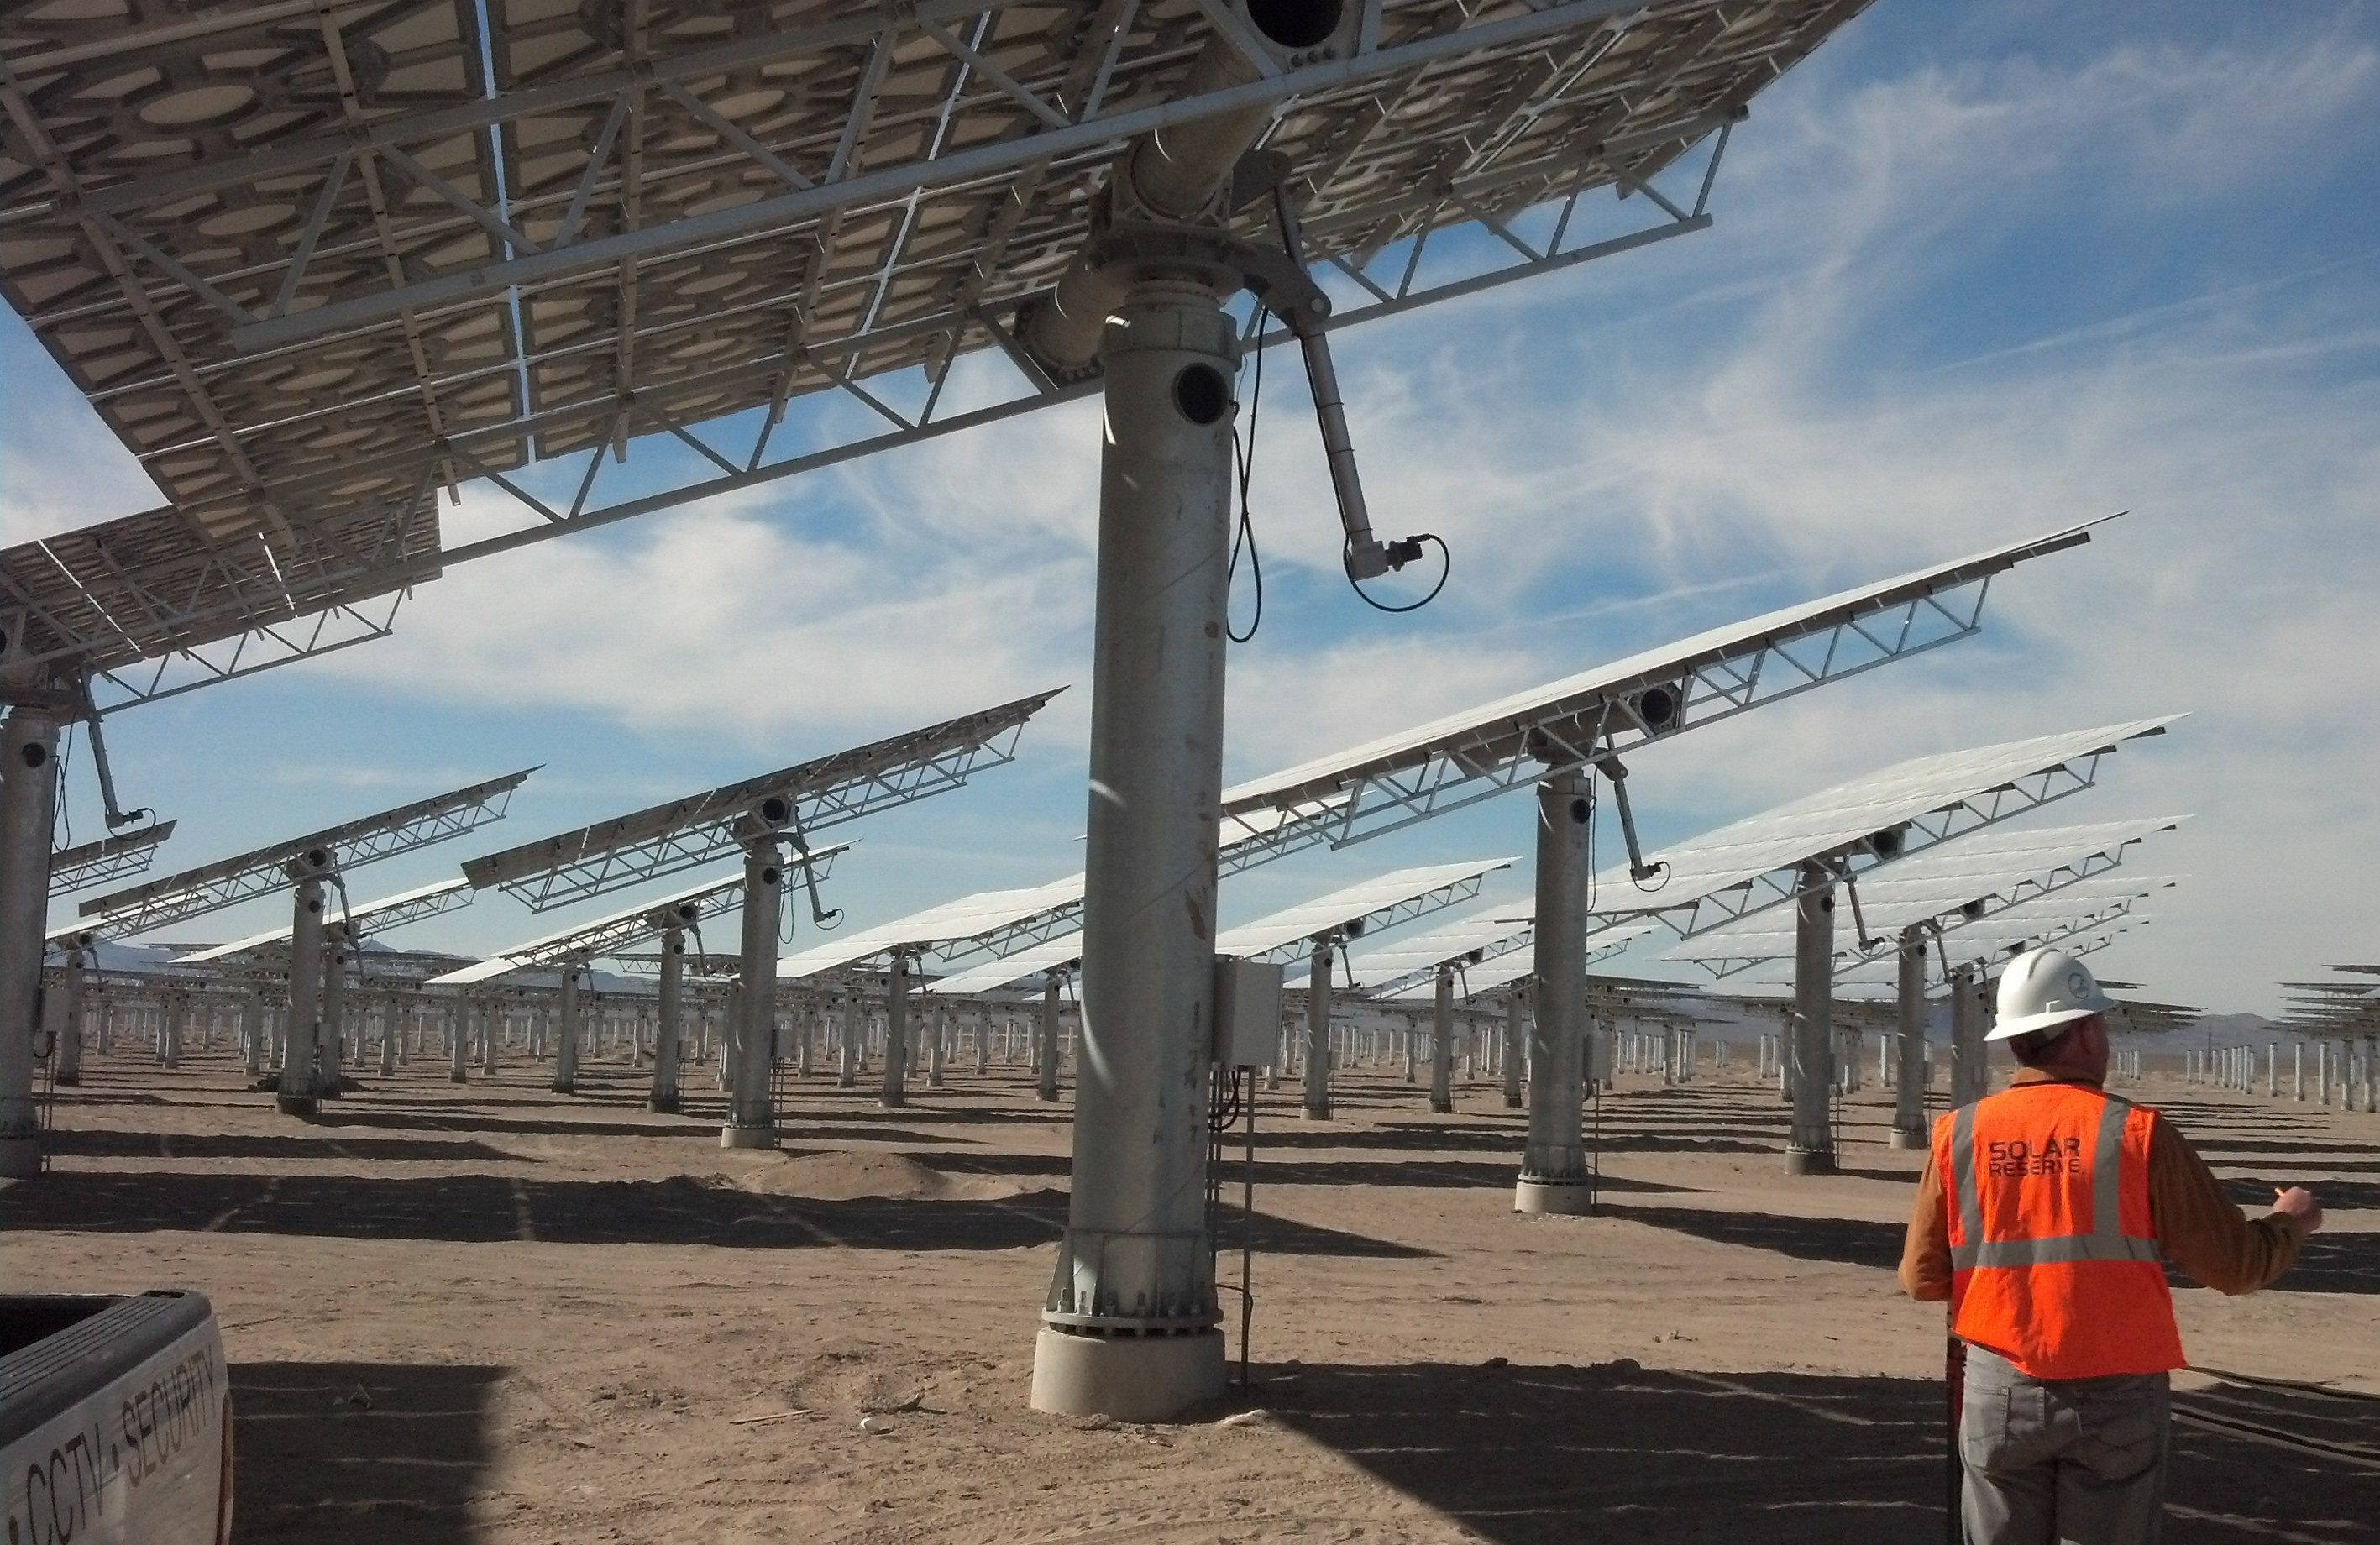
\includegraphics[width=.7\linewidth]{HeliostatImage.jpg}
\end{frame}

\begin{frame}
  \frametitle{As a Mechanical Engineer}
  \begin{itemize}
  \item Worked on the CDSEP plant performance model, integrating the Rocketdyne and Cobra code. (Fortran)
  \item Worked with the PV team on power project development
  \item Development of the PV performance model and design tool, and the systems engineering trades it allowed us to do quickly.
  \item Development of the CSP performance model/implementation of the smart dispatch logic in Matlab.
  \item Worked with the CSP team as well, mostly with Charles.
  \item Developed and troubleshot the financial model
  \item Although this was a spreadsheet, I ended up learning a bit about project finance and internal return calculation.
  \end{itemize}
\end{frame}

%% % All of the bullet points below deserve a slide
%% \begin{frame}
%%   \frametitle{As a Systems Engineer}
%%   \begin{itemize}
%%   \item Development of the SR-120 control software (Matlab)
%%   \item Kalman filter development
%%   \item Include some stuff about the "zero" finding logic?
%%   \item Development of the SVS-Vistek and ViewWorks camera interfaces in C#
%%   \item Test campaigns for the SR-120
%%   \item Determination and definition of performance requirements (IE mirror slope and pointing errors)
%%   \item Hands on testing at Sandia National Labs
%%   \item Troubleshooting and modifying the AMS software
%%   \item Camera and SPCA network setup 
%%   \item Daily SCRUMS (agile development) and piloting the system with Mark and Roger
%%   \item All of the performance data processing, which I had to automate because the rest of the team started on the SR-96
%%   \item Development of the in-situ/star characterization software
%%   \item Development of the control system interface; changing a relational object database into an object database
%%   \end{itemize}
%% \end{frame}

\subsection{Lockheed}

% I'm pretty sure this is copyrighted, so I shouldn't use it...
\begin{frame}
  \frametitle{Lockheed Martin Missiles and Fire Control}
  \center
  
\includegraphics[width=.7\linewidth]{LockheedLogo}
\end{frame}

\begin{frame}
  \frametitle{Affordability Test Bed}
  \begin{itemize}
  \item Describe what the ATB is and what it's intended to be
  \item Describe the loitering munition sim and the delay problem.
  \item Software overlay generation/frame numbers
  \item Camera triggering
  \item Describe the oscilloscope testing to determine 
  \item Display port $\rightarrow$ DVI $\rightarrow$ HDMI $\rightarrow$ VGA $\rightarrow$ BNC 5 wire (RGB + HSYNC + VSYNC) $\rightarrow$ Alligator clips
  \item Show the frame delay histogram
  \end{itemize}
\end{frame}


\begin{frame}
  \frametitle{PAC-3} % I might want to be a little sparing in my descriptions here, because this stuff is classified
  \begin{itemize}
  \item Which is intended to engage and destroy tactical ballistic missiles
  \item Most of it is classified
  \item Work on a Linux computing cluster on a continuous time simulation
  \item Integrating changes to the simulation from both internal, and also from the customer (IE the government), as well as the ground system components (which are from Raytheon).
  \item Integration of an older version of the simulation (entirely Fortran/Linux based) and modularizing it into several libraries which the customer can link together.  
  \item Builds on Windows or Linux
  \end{itemize}
\end{frame}

\begin{frame}
\Huge{\centerline{Q\&A}}
\end{frame}

\end{document} 
